%===================================== CHAP 1 =================================
\chapter{Introduction}

This chapter introduce the project, and will give overview 

\section{Background and Motivation} \label{sec:background}
The Construction Industry (CI) has been a significant part of engineering throughout history. Over the past century, the requirements of constructions have become more and more complex. The buildings are getting higher, the tunnels are getting longer, and the roads are getting wider. Sure, the size of things is not equal to the complexity of the construction; however, when considering automated systems, multipurpose functionality, and multiple communication platforms – the complexity is increasing. The increased complexity leads to a significant decline in labor productivity (LP), seen over the past two centuries, mentioned in the article written by SSB \cite{productivity}. As well, managing these projects is much more intricate then it used to, because of the increased numbers of actors participating in the project. 

One can argue that the negative progress in LP in the CI has to do with the increasing complexity, and therefore not a number to consider. Even so, better productivity and efficiency are always something management dicier, simply because of improved marginal cost.

The challenges the CI is experiencing, as well as the process used, are highly similar to what the ICT-industry was facing in the late '80s. The ICT-industry, using the waterfall process \cite{royce}, often faced the challenge of meeting the budgets and timelines. This breach had the origin in change of requirements during production, challenges in testing, and resultingly failing to deliver a finished product without bugs. These problems have been frequently present when creating large and highly user-interactive software — making for the introduction of agile software development to manage theses problems. Over the years, most of the process- and method-management in ICT is digitilized. Giving tools in which both the software developers and project managers use to aid project progression.  

Frank Garry, in 1997, first introduced 3-D modeling in CI, when constructing the Peter B. Lewis Building (PLB). 3-D modeling was used both to manage the complexity of the installation, but also led to increased cooperation between different parties within the project. The paper, describing this project \cite{frank_garry}, is reporting a change in how actors in the construction react to using computer-aided constructions, in 3-D. Today 3-D modeling is used in almost all construction projects and is known as BiM. Even though the PLB-project showed promising results in means of cooperation and interaction, the introduction of 3-D modeling was not a single solution to the problem.

Furthermore, one has introduced Lean in the CI. The book \cite{lean_i_praksis} describes the making of the Bergen Academy of Art and Design-building, where Lean was one of the essential strategies. The object of the Case Study in this research are using experience from this book when managing the constructions. 

The motivation for this rearch is to examine a project utilizing Lean in project management, to face the problems mentioned. Furthermore, looking at how a project make use of digital tools, aiding Lean has not been examined before. Taking experience from the ICT-industry, and the use of computer-aided agile development management is also desirable, as well as looking at the problem from a different perspective.

\section{Research and Question} \label{sec:research}
This project, therefore, aims to examine a case using Lean methodology, where digital tools are utilized to support both the methodology as well as cooperation and interaction between different actors.

{\bf $RQ1$: How and why are the project utilizing agile and lean methodology?}

{\bf $RQ1.1$: If any, what challenges is there using these methodologies?}

{\bf $RQ2$: Which digital tools are deployed in this project, aiding Lean Constructing, and how are they being used?}

{\bf $RQ2.1$: Are there any challenges making use of these digital tools?}

{\bf $RQ3$: Are there other factors that influence the use of project methodology or the digital tools used?}

\section{Deliverables} \label{sec:deliverables}
There will be three main deliverables in this thesis.

{\bf Literature review}: The first part of this research is a literature review on graphical passwords. A literature review is providing the information needed to decide on the main research hypothesis for my master thesis, and the aim is to fill the gap in research on graphical passwords on mobile devices.

{\bf Research design}: The gap found in the literature review will result in a problem domain to be worked in my master thesis. To be able to continue with this work, the research design for next semester will a deliverable of this work. The research design is mainly a detailed description of the research strategy and data collection method.

{\bf Empirical review}: Forklar


\section{Methods} \label{sec:methods}
\begin{figure}
    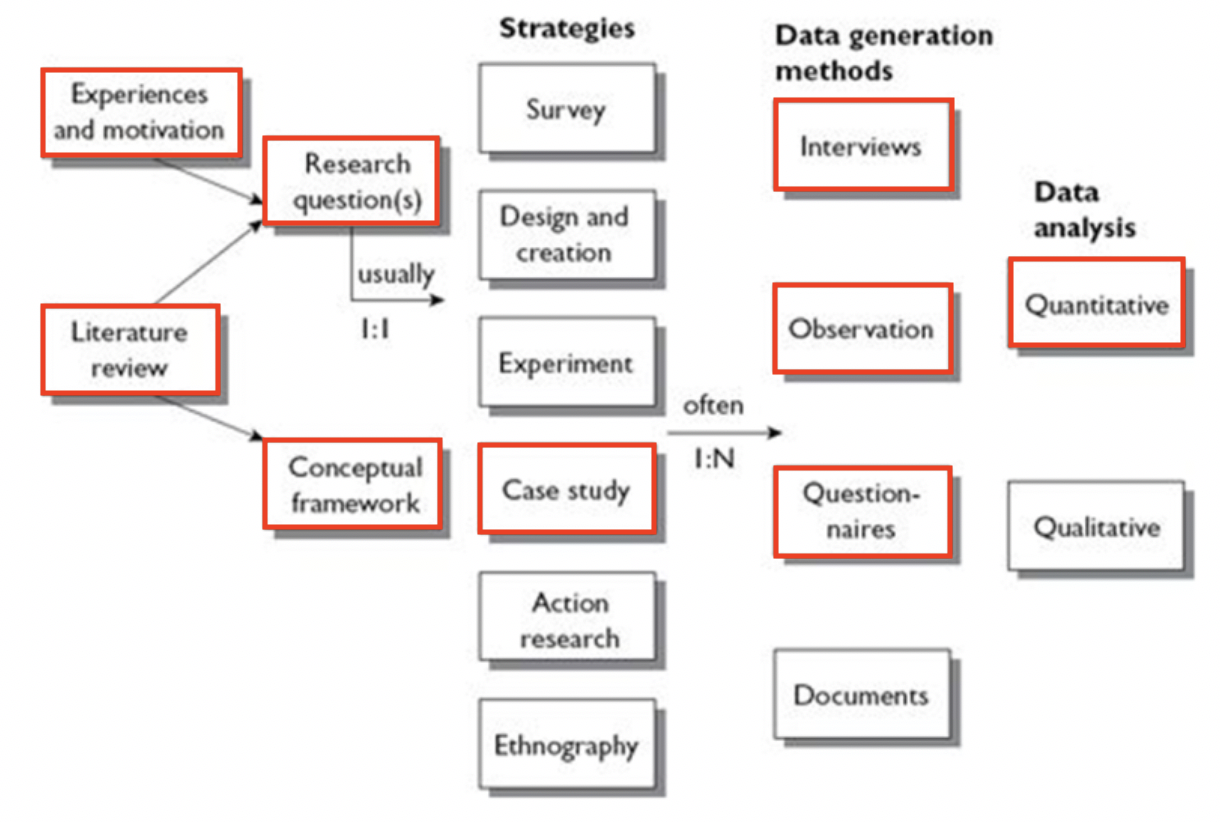
\includegraphics[width=\textwidth]{fig/empirisk_studie.png}
    \caption{The research process used, marked with methods applied in the research.}
    \label{fig:empirisk}
\end{figure}

This project originated in the interest in Software methodology, and how software aids productivity and cooperation in different parts of society. The projects formed when Patrick Stormo Hjerpseth, who is the Project Lead in Digitalization at the LSB-project, gave a tip regarding writing a master thesis about the LSB-project.

The project started with a literature review, providing a knowledgeable background for the project. Based on the literature review, one could see a clear correlation between software engineering (SE) 30 years ago and the construction engineering (CE) of today, as mentioned in the purpose section. To identify how these problems can be faced in a project, using agile management methods and CSCW, the master thesis is planning a case study-strategy. The case studied is the LSB-project. 

First, the research will do a minor empirical study in the project thesis, utilizing observation and interviews as data generators. This research will hopefully give insights that will bring the research to a narrower focus on the following master thesis. 

Secondary, in the master thesis, conduction of interviews and a questionnaire will aid the analysis as data generation methods. If necessary, observations will be conducted. The questionnaire will give questions on a standardized format that can be valuable in the analyses. Furthermore, the interviews will help to discover matters not covered in the questionnaire. Both interviews, the questionnaires, and observations will give quantitative data for the analysis.
\section{Litterature review} \label{sec:litterature}
Forklar outline av innholdet
\section{Thesis structure} \label{sec:thesis}

{\bf Chapter 2: Literature Review} provides an overview of 

{\bf Chapter 3: Empirical Review}

{\bf Chapter 5: Analysis and Discussion}

{\bf Chapter 4: Research Design} present the chosen research strategy and data collection method that will be used in my master thesis. 

{\bf Chapter 5: Further Work} 

\cleardoublepage